% Generated by Sphinx.
\documentclass[letterpaper,10pt,ngerman]{manual}
\usepackage[utf8]{inputenc}
\usepackage[T1]{fontenc}
\usepackage{babel}
\usepackage{times}
\usepackage[Sonny]{fncychap}
\usepackage{longtable}
\usepackage{sphinx}


\title{BNG Bootloader Documentation}
\date{20. 04. 2010}
\release{0.2}
\author{Elias Medawar, Yves Peissard, Simon Honegger, Jonathan Stoppani}
\newcommand{\sphinxlogo}{}
\renewcommand{\releasename}{Release}
\makeindex
\makemodindex

\makeatletter
\def\PYG@reset{\let\PYG@it=\relax \let\PYG@bf=\relax%
    \let\PYG@ul=\relax \let\PYG@tc=\relax%
    \let\PYG@bc=\relax \let\PYG@ff=\relax}
\def\PYG@tok#1{\csname PYG@tok@#1\endcsname}
\def\PYG@toks#1+{\ifx\relax#1\empty\else%
    \PYG@tok{#1}\expandafter\PYG@toks\fi}
\def\PYG@do#1{\PYG@bc{\PYG@tc{\PYG@ul{%
    \PYG@it{\PYG@bf{\PYG@ff{#1}}}}}}}
\def\PYG#1#2{\PYG@reset\PYG@toks#1+\relax+\PYG@do{#2}}

\def\PYG@tok@gd{\def\PYG@tc##1{\textcolor[rgb]{0.63,0.00,0.00}{##1}}}
\def\PYG@tok@gu{\let\PYG@bf=\textbf\def\PYG@tc##1{\textcolor[rgb]{0.50,0.00,0.50}{##1}}}
\def\PYG@tok@gt{\def\PYG@tc##1{\textcolor[rgb]{0.00,0.25,0.82}{##1}}}
\def\PYG@tok@gs{\let\PYG@bf=\textbf}
\def\PYG@tok@gr{\def\PYG@tc##1{\textcolor[rgb]{1.00,0.00,0.00}{##1}}}
\def\PYG@tok@cm{\let\PYG@it=\textit\def\PYG@tc##1{\textcolor[rgb]{0.25,0.50,0.56}{##1}}}
\def\PYG@tok@vg{\def\PYG@tc##1{\textcolor[rgb]{0.73,0.38,0.84}{##1}}}
\def\PYG@tok@m{\def\PYG@tc##1{\textcolor[rgb]{0.13,0.50,0.31}{##1}}}
\def\PYG@tok@mh{\def\PYG@tc##1{\textcolor[rgb]{0.13,0.50,0.31}{##1}}}
\def\PYG@tok@cs{\def\PYG@tc##1{\textcolor[rgb]{0.25,0.50,0.56}{##1}}\def\PYG@bc##1{\colorbox[rgb]{1.00,0.94,0.94}{##1}}}
\def\PYG@tok@ge{\let\PYG@it=\textit}
\def\PYG@tok@vc{\def\PYG@tc##1{\textcolor[rgb]{0.73,0.38,0.84}{##1}}}
\def\PYG@tok@il{\def\PYG@tc##1{\textcolor[rgb]{0.13,0.50,0.31}{##1}}}
\def\PYG@tok@go{\def\PYG@tc##1{\textcolor[rgb]{0.19,0.19,0.19}{##1}}}
\def\PYG@tok@cp{\def\PYG@tc##1{\textcolor[rgb]{0.00,0.44,0.13}{##1}}}
\def\PYG@tok@gi{\def\PYG@tc##1{\textcolor[rgb]{0.00,0.63,0.00}{##1}}}
\def\PYG@tok@gh{\let\PYG@bf=\textbf\def\PYG@tc##1{\textcolor[rgb]{0.00,0.00,0.50}{##1}}}
\def\PYG@tok@ni{\let\PYG@bf=\textbf\def\PYG@tc##1{\textcolor[rgb]{0.84,0.33,0.22}{##1}}}
\def\PYG@tok@nl{\let\PYG@bf=\textbf\def\PYG@tc##1{\textcolor[rgb]{0.00,0.13,0.44}{##1}}}
\def\PYG@tok@nn{\let\PYG@bf=\textbf\def\PYG@tc##1{\textcolor[rgb]{0.05,0.52,0.71}{##1}}}
\def\PYG@tok@no{\def\PYG@tc##1{\textcolor[rgb]{0.38,0.68,0.84}{##1}}}
\def\PYG@tok@na{\def\PYG@tc##1{\textcolor[rgb]{0.25,0.44,0.63}{##1}}}
\def\PYG@tok@nb{\def\PYG@tc##1{\textcolor[rgb]{0.00,0.44,0.13}{##1}}}
\def\PYG@tok@nc{\let\PYG@bf=\textbf\def\PYG@tc##1{\textcolor[rgb]{0.05,0.52,0.71}{##1}}}
\def\PYG@tok@nd{\let\PYG@bf=\textbf\def\PYG@tc##1{\textcolor[rgb]{0.33,0.33,0.33}{##1}}}
\def\PYG@tok@ne{\def\PYG@tc##1{\textcolor[rgb]{0.00,0.44,0.13}{##1}}}
\def\PYG@tok@nf{\def\PYG@tc##1{\textcolor[rgb]{0.02,0.16,0.49}{##1}}}
\def\PYG@tok@si{\let\PYG@it=\textit\def\PYG@tc##1{\textcolor[rgb]{0.44,0.63,0.82}{##1}}}
\def\PYG@tok@s2{\def\PYG@tc##1{\textcolor[rgb]{0.25,0.44,0.63}{##1}}}
\def\PYG@tok@vi{\def\PYG@tc##1{\textcolor[rgb]{0.73,0.38,0.84}{##1}}}
\def\PYG@tok@nt{\let\PYG@bf=\textbf\def\PYG@tc##1{\textcolor[rgb]{0.02,0.16,0.45}{##1}}}
\def\PYG@tok@nv{\def\PYG@tc##1{\textcolor[rgb]{0.73,0.38,0.84}{##1}}}
\def\PYG@tok@s1{\def\PYG@tc##1{\textcolor[rgb]{0.25,0.44,0.63}{##1}}}
\def\PYG@tok@gp{\let\PYG@bf=\textbf\def\PYG@tc##1{\textcolor[rgb]{0.78,0.36,0.04}{##1}}}
\def\PYG@tok@sh{\def\PYG@tc##1{\textcolor[rgb]{0.25,0.44,0.63}{##1}}}
\def\PYG@tok@ow{\let\PYG@bf=\textbf\def\PYG@tc##1{\textcolor[rgb]{0.00,0.44,0.13}{##1}}}
\def\PYG@tok@sx{\def\PYG@tc##1{\textcolor[rgb]{0.78,0.36,0.04}{##1}}}
\def\PYG@tok@bp{\def\PYG@tc##1{\textcolor[rgb]{0.00,0.44,0.13}{##1}}}
\def\PYG@tok@c1{\let\PYG@it=\textit\def\PYG@tc##1{\textcolor[rgb]{0.25,0.50,0.56}{##1}}}
\def\PYG@tok@kc{\let\PYG@bf=\textbf\def\PYG@tc##1{\textcolor[rgb]{0.00,0.44,0.13}{##1}}}
\def\PYG@tok@c{\let\PYG@it=\textit\def\PYG@tc##1{\textcolor[rgb]{0.25,0.50,0.56}{##1}}}
\def\PYG@tok@mf{\def\PYG@tc##1{\textcolor[rgb]{0.13,0.50,0.31}{##1}}}
\def\PYG@tok@err{\def\PYG@bc##1{\fcolorbox[rgb]{1.00,0.00,0.00}{1,1,1}{##1}}}
\def\PYG@tok@kd{\let\PYG@bf=\textbf\def\PYG@tc##1{\textcolor[rgb]{0.00,0.44,0.13}{##1}}}
\def\PYG@tok@ss{\def\PYG@tc##1{\textcolor[rgb]{0.32,0.47,0.09}{##1}}}
\def\PYG@tok@sr{\def\PYG@tc##1{\textcolor[rgb]{0.14,0.33,0.53}{##1}}}
\def\PYG@tok@mo{\def\PYG@tc##1{\textcolor[rgb]{0.13,0.50,0.31}{##1}}}
\def\PYG@tok@mi{\def\PYG@tc##1{\textcolor[rgb]{0.13,0.50,0.31}{##1}}}
\def\PYG@tok@kn{\let\PYG@bf=\textbf\def\PYG@tc##1{\textcolor[rgb]{0.00,0.44,0.13}{##1}}}
\def\PYG@tok@o{\def\PYG@tc##1{\textcolor[rgb]{0.40,0.40,0.40}{##1}}}
\def\PYG@tok@kr{\let\PYG@bf=\textbf\def\PYG@tc##1{\textcolor[rgb]{0.00,0.44,0.13}{##1}}}
\def\PYG@tok@s{\def\PYG@tc##1{\textcolor[rgb]{0.25,0.44,0.63}{##1}}}
\def\PYG@tok@kp{\def\PYG@tc##1{\textcolor[rgb]{0.00,0.44,0.13}{##1}}}
\def\PYG@tok@w{\def\PYG@tc##1{\textcolor[rgb]{0.73,0.73,0.73}{##1}}}
\def\PYG@tok@kt{\def\PYG@tc##1{\textcolor[rgb]{0.56,0.13,0.00}{##1}}}
\def\PYG@tok@sc{\def\PYG@tc##1{\textcolor[rgb]{0.25,0.44,0.63}{##1}}}
\def\PYG@tok@sb{\def\PYG@tc##1{\textcolor[rgb]{0.25,0.44,0.63}{##1}}}
\def\PYG@tok@k{\let\PYG@bf=\textbf\def\PYG@tc##1{\textcolor[rgb]{0.00,0.44,0.13}{##1}}}
\def\PYG@tok@se{\let\PYG@bf=\textbf\def\PYG@tc##1{\textcolor[rgb]{0.25,0.44,0.63}{##1}}}
\def\PYG@tok@sd{\let\PYG@it=\textit\def\PYG@tc##1{\textcolor[rgb]{0.25,0.44,0.63}{##1}}}

\def\PYGZbs{\char`\\}
\def\PYGZus{\char`\_}
\def\PYGZob{\char`\{}
\def\PYGZcb{\char`\}}
\def\PYGZca{\char`\^}
% for compatibility with earlier versions
\def\PYGZat{@}
\def\PYGZlb{[}
\def\PYGZrb{]}
\makeatother

\begin{document}
\shorthandoff{"}
\maketitle
\tableofcontents
\hypertarget{--doc-index}{}

\hypertarget{todo-2}{}
\resetcurrentobjects
\hypertarget{--doc-abstract}{}

\chapter{Abstract}

Dieses Projekt hat zum Ziel im Ramen des Kurses ``Mikroprozessoren 2''
der Hochschule für Technik und Architektur einen Bootloader auf einem
Mikrochip MC68332 zu implementieren. Dabei werden die behandelten Themen
des Mikroprozessor Kurses \emph{Programmieren in C} und \emph{Grundlagen Assembler}
angewendet. Nach Aufstarten des Mikrokontrollers kann eine externe Maschine
(Terminal) mittels serieller Schnittstelle angeschlossen werden, mit der
anschliessend Befehle eingegeben werden können um den Bootloader zu
konfigurieren. Der Benutzer soll schliesslich unter zwei verschiedenen
Anwendungen auswählen können, die er mit dem Bootloader starten will.

Was ist ein \emph{Bootloader}?
Definition von Wikipedia: Ein Bootloader ist eine spezielle Software, die gewöhnlich durch
die Firmware  (z. B. dem BIOS bei IBM-kompatiblen PCs) eines Rechners von
einem bootfähigen Medium geladen und anschließend ausgeführt wird. Der
Bootloader lädt dann weitere Teile des Betriebssystems, gewöhnlich einen
Kernel.

\resetcurrentobjects
\hypertarget{--doc-architecture/index}{}

\chapter{Architektur}


\section{Überblick}

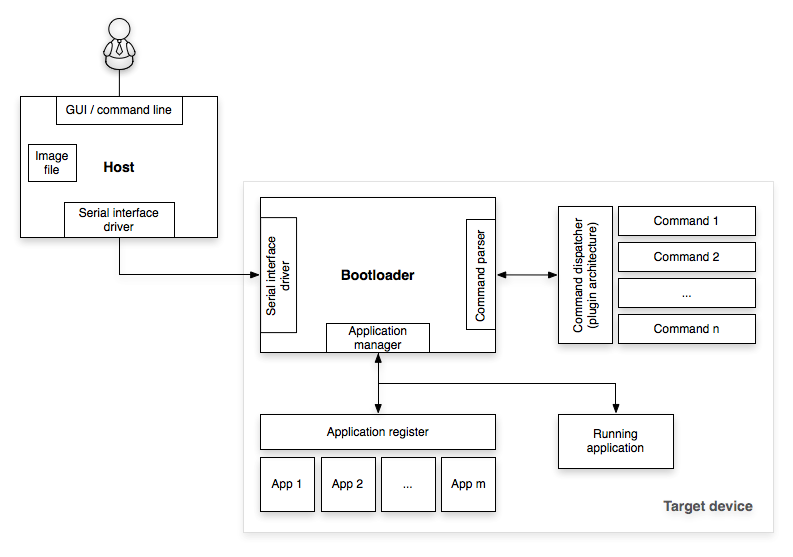
\includegraphics{overview.png}

In der obenstehenden Gesammtübersicht sind die einzelnen Komponenten und deren Verknüpfung dargestellt.
Im folgenden Kapitel wird die Architektur der jeweiligen Komponenten näher
beschrieben.


\section{Application Driver}

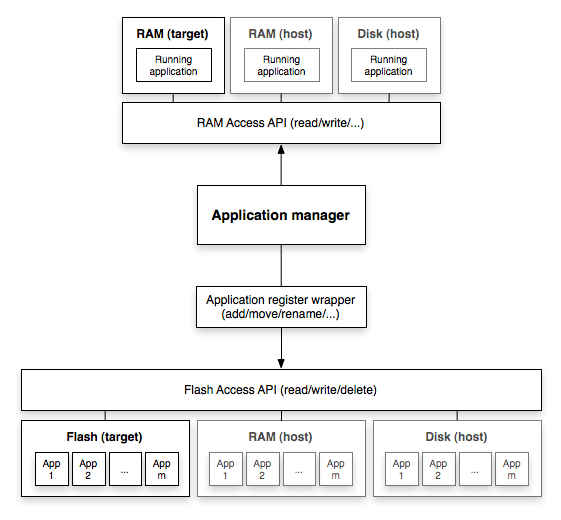
\includegraphics{app-manager.png}

Die Aufgabe der Application Driver ist es, das Applikationsverzeichnis zu
verwalten und den aktuellen Ihnalt des Flashspeichers in den Arbeitsspeicher zu laden.


\subsection{Flash Access API}

Mit der Flash Access API können entweder Flashspeicher, Arbeitsspeicher oder
Festplatte benutzt werden. Die drei Hauptfunktionen der API sind lesen,
schreiben und löschen.
Der Zugriff auf den Flashspeicher ist nur mittels Mikrokontroller MC68332 möglich (Zielplattform).
Lesen und/oder Schreiben auf Arbeitsspeicher oder Festplatte sind für Testzwecke gedacht (Debugging).


\subsection{Application Register Wrapper}

Damit nicht direkt mit der Flash API gearbeitet werden muss, übernimmt der
Application Register Wrapper die Ansteuerung der Flash Access API. Dies
erleichtert das Entwickeln des Bootloaders und ermöglicht den Code des
Application Driver übersichtlich zu gestalten.


\section{Serial Interface Driver}

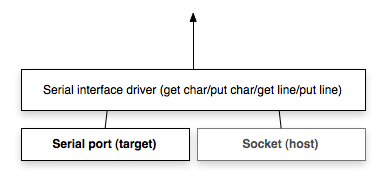
\includegraphics{serial-driver.png}

Der Serial Interface Driver ermöglicht die Kommunikation zwischen Zielplattform (MC68332)
und Benutzer des Bootloader. Mittels eines Keyboards und einem Terminal werden
Zeichen an den Mikrokontroller geschickt und das Resultat vom Kontroller
anschliessend wieder an den Benutzer zurück geschickt. Funktionen wie
put\_char oder get\_char müssen hier implementiert werden.
Damit wir die Serielle Schnittstelle in unserer Testumbebung emulieren können werden wir ein Socket benutzen.


\section{Command Parser}

Der Command Parser analysiert die einkommenden Befehle des Benutzerkeyboards
und delegiert das Aufrufen der entsprechenden Methoden (siehe Commands).

\resetcurrentobjects
\hypertarget{--doc-specification/index}{}

\chapter{Spezifikation}

\resetcurrentobjects
\hypertarget{--doc-specification/specification}{}

\section{Anforderungsspezifikation}


\subsection{Funktional}


\subsubsection{Muss}

Muss Ziele sind von der Projektspezifikation gegeben und müssen erfüllt werden.
\begin{enumerate}
\item {} 
Nach einschalten der Hardware wird der Bootloader automatisch gestartet

\item {} 
Der Bootloader muss eine Applikation aufnehmen und diese permanent speichern;

\item {} 
Der Bootloader muss eine permanente Applikation starten;

\item {} 
Der Benutzer muss eine exisitierende Applikation entfernen;

\item {} 
Binärdaten des Formats S-Record können behandelt werden;

\item {} 
Der Bootloader hat keine Auswirkung auf die funktionsweise der auszuführenden Applikation.

\end{enumerate}


\subsubsection{Kann}
\begin{enumerate}
\item {} 
Der Bootloader zeigt eine Auswahl an zu verfügung stehenden Applikation an;

\item {} 
Der Bootloader started nach einer gewissen Zeit eine vom Benutzer als default markierte Applikation;

\item {} 
Eine Applikation kann auf das Gerät geladen werden ohne es permanent zu speichern;
Dies auch wenn der Speicherplatz des permanenten Specihers belegt ist. Dieses kann ausgeführt werden;
Bei Neustart des Geräts ist dieses nicht mehr vorhanden. Nach nicht permanenten laden einer Applikation;
ist der vorherige Zustand nach dem neustarten wieder hergestellt;

\item {} 
Nach permanentem speichern einer Applikation und späterer Löschung ist der Zustand für den Anwender unverändert;

\item {} 
Der Speicherplatz wird insofern optimal genutzt, dass keine unnötigen, nicht verwendbaren Lücken enstehen;

\item {} 
Es kann eine default Applikation gewählt werden, welche nach einem gewissen Timeout automatisch gestartet wird;

\item {} 
Eine default Applikation wird nicht mehr als 5 mal hintereinander autmatisch gestartet, falls dessen verarbeitung fehlerhaft war;

\end{enumerate}


\subsection{Nicht-Funktional}
\begin{enumerate}
\item {} 
Der Code sowie Kommentar sind in englisch gehalten;

\item {} 
Der Source code muss dokumentiert sein;

\item {} 
Ein Nutzer mit shell Kentnissen kommt mit der Benutzerschnittstelle zurecht. D. h., das Grundprinzip des Eingebens
von verschiedenen Kommandos und deren Parameter, sowie die Benutzung des ``Hilfe'' Befehls sollte dem Benutzer vertraut sein.

\end{enumerate}

\resetcurrentobjects
\hypertarget{--doc-specification/commands}{}

\section{Befehle}
\hypertarget{todo-3}{}
\code{help}
\begin{quote}

Zeigt eine Liste aller möglichen Befehle an.
\end{quote}


\bigskip\hrule{}\bigskip


\code{help command-name}
\begin{quote}

Zeigt die Hilfe für \code{command-name} an.
\end{quote}


\bigskip\hrule{}\bigskip


\code{download {[}-b app-name {[}-d{]}{]}}
\begin{quote}

Lädt die folgenden Daten in den Arbeitsspeicher als eine SRecord Datei.
\begin{optionlist}{3cm}
\item [-b app-id]  
Führt den Befehl \code{burn app-id} aus.
\item [-d]  
Setzt die Applikation als default Startanwendung
\end{optionlist}
\end{quote}


\bigskip\hrule{}\bigskip


\code{burn app-name {[}-d{]}}
\begin{quote}

Speichert das sich im Arbeitsspeicher befindende SRecordFile in den Flashspeicher unter dem Namen \code{app-name}.
\begin{optionlist}{3cm}
\item [-d]  
Setzt die zu brennende Applikation als default Startanwendung
\end{optionlist}
\end{quote}


\bigskip\hrule{}\bigskip


\code{run {[}-r\textbar{}app-id{]}}
\begin{quote}

Führt die default, oder die mit dem \code{app-id} identifizierte Applikation aus.
\begin{optionlist}{3cm}
\item [-r]  
Führt das sich im Arbeitsspeicher befindende SRecordFile aus.
\end{optionlist}
\end{quote}


\bigskip\hrule{}\bigskip


\code{list}
\begin{quote}

Führt eine Liste der sich im Flashspeicher befindenden Applikationen auf.
\end{quote}


\bigskip\hrule{}\bigskip


\code{set {[}-{-}default=app-id{]} {[}-{-}timeout=seconds{]} {[}...{]}}
\begin{quote}

Setzt die Werte der gegebenen Konfigurationsoptionen.
\begin{optionlist}{3cm}
\item [-d app-id]  
Siehe \code{-{-}default-app}
\item [-{-}default=app-id]  
Setzt die default Applikation
\item [-t seconds]  
Siehe \code{-{-}default-app}
\item [-{-}timeout=seconds]  
Setzt die Wartezeit nach der die default Applikation gestartet werden soll
\item [-e num]  
Siehe \code{-{-}default-app}
\item [-{-}errcount=num]  
Anzahl Neustarts im Falle eines fehlerhafen Starts einer Applikation.
Sobald errorcount erreicht ist, wird das Timeout deaktiviert und den Bootloader wird in Terminal-Mode umschalten.
\end{optionlist}
\end{quote}


\bigskip\hrule{}\bigskip


\code{bootconfig}
\begin{quote}

Führt die aktuelle Konfiguration (app-name, timeout, errorcount) des Bootloaders auf.
\end{quote}


\bigskip\hrule{}\bigskip


\code{erase app-id}
\begin{quote}

Entfernt die mit dem \code{app-id} identifizierte Applikation aus der Applikationsliste des Flashspeichers.
\end{quote}

\resetcurrentobjects
\hypertarget{--doc-appendices/index}{}

\chapter{Anlagen}


\section{Anlage 1: Planung}

Das folgende Bild zeigt die Großplanung für das Bootloader Projekt. Diese Planung wird während der Entwicklung kontinuierlich aktualisiert.

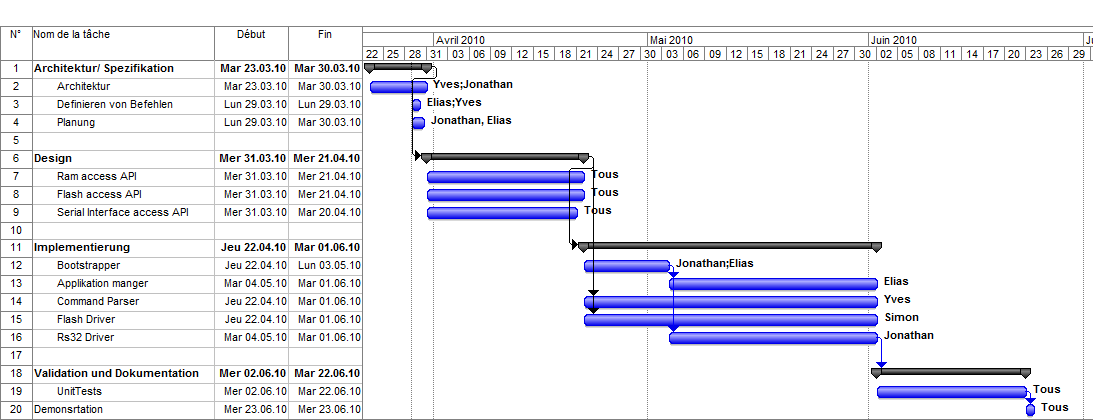
\includegraphics{planung.png}

Ein (Druck-geeignetes) PDF und das originale MS Project Dokument sind auch verfügbar:
\begin{itemize}
\item {} 
Planung PDF Dokument

\item {} 
Planung MS Project Dokument

\end{itemize}


\section{Anlage 2: Entwicklungs-prozess}

Das ganze Projekt wird auf github (\href{http://github.com}{http://github.com}) verwaltet.
\begin{itemize}
\item {} 
Git Repository auf github: \href{http://github.com/garetjax/Bootloader}{http://github.com/garetjax/Bootloader}

\end{itemize}
\hypertarget{todo-0}{}

\section{Anlage 3: Ressourcen}


\subsection{Interne ressourcen}
\begin{itemize}
\item {} 
HTML Build der dokumentation: \href{http://garetjax.github.com/Bootloader}{http://garetjax.github.com/Bootloader}

\item {} 
HTML Build der spezifikation: \href{http://garetjax.github.com/Bootloader/api/}{http://garetjax.github.com/Bootloader/api/}

\item {} 
PDF Build der dokumentation: \href{http://garetjax.github.com/Bootloader/static/documentation.pdf}{http://garetjax.github.com/Bootloader/static/documentation.pdf}

\item {} 
PDF Build der spezifikation: \href{http://garetjax.github.com/Bootloader/static/api.pdf}{http://garetjax.github.com/Bootloader/static/api.pdf}

\end{itemize}


\subsection{Externe ressourcen}
\begin{itemize}
\item {} 
Git: \href{http://git-scm.com/}{http://git-scm.com/}

\item {} 
Sphinx: \href{http://sphinx.pocoo.org}{http://sphinx.pocoo.org}

\item {} 
Doxygen: \href{http://www.stack.nl/~dimitri/doxygen/}{http://www.stack.nl/\textasciitilde{}dimitri/doxygen/}

\end{itemize}


\section{Anlage 4: Referenzen}
\hypertarget{todo-1}{}

\section{Anlage 3: TODOs}

Sphinx ermöglicht das direkte Einfügen von \emph{zu tun} Elemente in der Dokumentation.
Diese Elemente können während des Builds durch eine Konfigurationsoption ausgeblendet werden.

Um ein neues \emph{zu tun} Element hinzuzufügen, ist die folgende Syntax zu verwenden:

\begin{Verbatim}[commandchars=@\[\]]
.. todo::
   A simple text describing what we have to do.
   * But it could be
   * a list too
   * if the points are many
\end{Verbatim}

Diese Elemente können durch die folgende Syntax in einer Auflistung zusammengefasst werden:

\begin{Verbatim}[commandchars=@\[\]]
.. todolist::
\end{Verbatim}

Hier unten sind alle, in der Dokumentation gefundene, \emph{zu tun} Element aufgelistet (falls sie aktiviert sind).


\renewcommand{\indexname}{Modulindex}
\printmodindex
\renewcommand{\indexname}{Stichwortverzeichnis}
\printindex
\end{document}
